\chapter{Redmine}\label{chp:redmine}

\section{Introdução}\label{sec:redmine-introducao}

Criado em 2006 por Jean-Philippe Lang, o Redmine\cite{redmine} pode ser definido como uma aplicação \textit{web} desenvolvida para o gerenciamento de projetos. Desenvolvido na linguagem de programação Ruby\cite{ruby-lang}, utiliza a \textit{framework} Rails\cite{rails} para suportar sua arquitetura \textit{web}. Conforme apresentado no livro Mastering Redmine\cite{mastering_redmine}, este sistema pode ser considerado um dos carros-chefes em soluções para a gestão de projetos no mundo \textit{open-source}.

Neste capítulo vamos explicar como o Redmine, uma ferramenta criada inicialmente para a gestão de projetos, foi utilizada para gestão de processos. Vamos apresentar também, a capacidade extensiva desta ferramenta através do desenvolvimento de \textit{plugins}. Por último, vamos abordar as limitações do Redmine que nos motivaram a buscar novas alternativas, e com isso atingir um estágio mais avançado na automatização de processos.

\section{Estrutura básica do Redmine}\label{sec:redmine-estrutura_basica}

A estrutura básica de gerenciamento de projetos no Redmine é composta por 6 principais elementos. São eles:

\subsection{Projetos}\label{subsection:redmine-estrutura_basica-projeto}

Projetos são o objeto central do Redmine. Eles são compostos por diversos módulos que acrescentam diferentes dimensões para o seu gerenciamento, como gerenciamento de tarefas, planejamento de etapas e marcos no projeto, acompanhamento do progresso das tarefas em um diagrama de \textit{Gantt}, \textit{Wiki} para organização do conhecimento, entre outros. 

\subsection{Tarefas}\label{subsection:redmine-estrutura_basica-tarefa}

São as unidades básicas de execução de trabalho dos projetos (\ref{subsection:redmine-estrutura_basica-projeto}). Elas contêm os dados relevantes para o seu gerenciamento (e.g, tipo (\ref{subsection:redmine-estrutura_basica-tracker}), situação (\ref{subsection:redmine-estrutura_basica-status})), e a sua execução (e.g, título, descrição) e dados adicionais que podem variar entre os projetos e tipos de tarefa, os quais são cadastrados como campos personalizados (\ref{subsection:redmine-estrutura_basica-custom_fields}). É possível criar uma pequena hierarquia de tarefas, que chamaremos de sub-tarefa, quando uma tarefa é relacionada a outra.

\subsection{Tipos de tarefa}\label{subsection:redmine-estrutura_basica-tracker}

Tipos de tarefa definem o fluxo de trabalho para a realização de atividades similares. De acordo com o tipo, variam as informações necessárias para a execução da tarefa, a sequência de passos para sua conclusão e as ações que cada membro do projeto pode desempenhar em cada etapa.

\subsection{Papéis de usuários}\label{subsection:redmine-estrutura_basica-role}

Os papéis de usuários definem quais permissões um usuário possui, como, por exemplo, visualizar, adicionar e editar tarefas, editar \textit{Wiki}, adicionar e editar documentos. Os papéis são atribuídos aos usuários em cada projeto que ele participa, portanto, ele pode possuir permissões diferentes dependendo do projeto de que ele é membro. A Figura \ref{fig:redmine_papeis} ilustra a tela aonde a configuração das permissões de um papel é feita.

\begin{figure}[H]
  \centering
  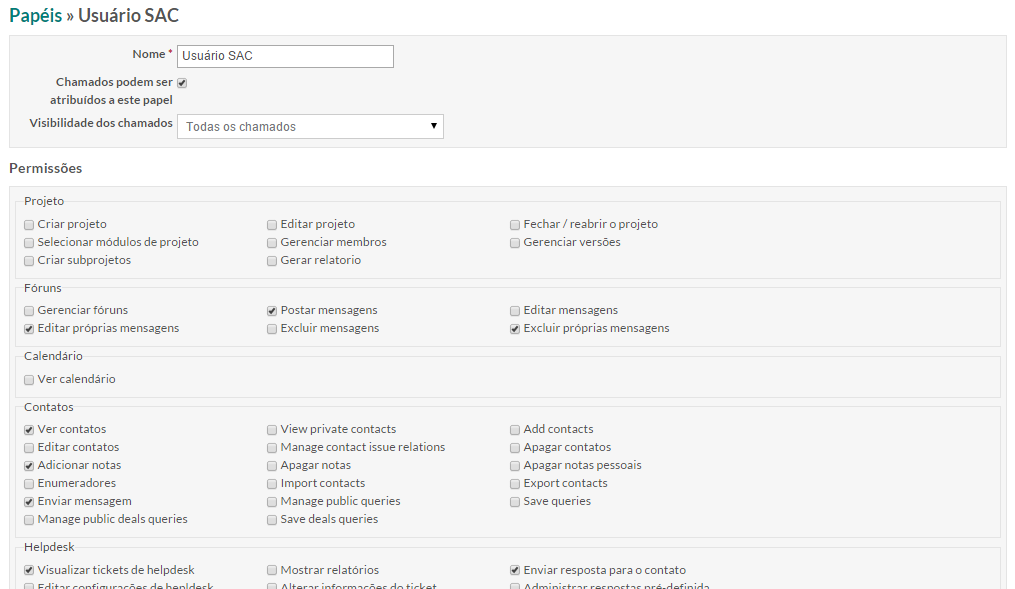
\includegraphics[width=1.0\textwidth]{imagens/redmine_papeis.png}
  \caption{Tela de configuração das permissões de um papel}
  \label{fig:redmine_papeis}
\end{figure}

\subsection{Situação das tarefas}\label{subsection:redmine-estrutura_basica-status}

Situação indica em qual etapa do processo uma tarefa se encontra, como "Novo", "Em andamento", "Concluído". Na tela de fluxo de trabalho é possível configurar, para cada papel de usuário, tipo de tarefa e situação, quais campos do formulário podem ser visualizados, ou editados.

\subsection{Campos personalizados}\label{subsection:redmine-estrutura_basica-custom_fields}

Todas as tarefas de projetos possuem dados em comum, como data de início, data de término e descrição. No entanto, dependendo das especificidades de um projeto ou tipo de tarefa, podem ser necessárias informações adicionais. Para esses casos existem os campos personalizados. Eles permitem criar novos campos e adicioná-los às tarefas, estendendo as configurações padrão da ferramenta.

\section{Gestão de processos com o Redmine}\label{sec:redmine-gestao_processos}

A estrutura de projetos do Redmine é altamente configurável. Todos os elementos explicados na seção \ref{sec:redmine-estrutura_basica} são cadastrados pelos usuários administradores do sistema que são responsáveis por configurá-los e personalizá-los para atender às demandas de cada projeto.

Todas as configurações e personalizações citadas no último parágrafo são feitas exclusivamente pela interface da ferramenta, sem necessidade de alterações no código da aplicação ou arquivos de configuração, o que confere aos administradores capacidade para modelar a estrutura da ferramenta da forma que for mais conveniente para a necessidade dos usuários.

Além disso, o módulo de gerenciamento de tarefas permite ao usuário interagir muito bem com o projeto, tendo total controle de suas tarefas, e ainda submetido a um controle de acesso bem detalhado e flexível.

As vantagens citadas acima, e ainda o fato de o Redmine ser \textit{open-source}, com uma grande comunidade de usuários e desenvolvedores foram motivadoras para a utilização deste como um gerenciador de processos.

\section{Modelando processos com o Redmine}\label{sec:redmine-automatizar_processo}

O primeiro passo para modelar um processo é identificar como representá-lo na estrutura do Redmine.

Nesta seção, descreveremos como utilizar o potencial de configuração do Redmine para utilizá-lo fora do contexto de gerenciamento de projetos e aplicá-lo como ferramenta de automatização de processos. Explicaremos, também, como definir os atores de um processo, as ações permitidas a cada um deles, especificar os fluxos de trabalho e como gerenciar os dados relevantes ao seu contexto. Estes passos serão ilustrados na implementação do caso de uso descrito na seção \ref{sec:introducao-caso_real}

\subsection{Modelando processos}\label{subsection:redmine-automatizar_processo-criacao}

Para modelar um processo no Redmine, utilizamos os \underline{tipos de tarefa} (\ref{subsection:redmine-estrutura_basica-tracker}) para estruturar os diferentes processos que podem ser iniciados. Durante a criação do tipo de tarefa, define-se qual situação (\ref{subsection:redmine-estrutura_basica-status}) é a padrão para aquele tipo, em quais projetos ele é utilizado e quais campos (\ref{subsection:redmine-estrutura_basica-custom_fields}) ele utiliza para guardar informações. Os \underline{projetos} são utilizados para agrupar processos da forma desejada. As \underline{tarefas} (\ref{subsection:redmine-estrutura_basica-tarefa}) são utilizadas para representar instâncias de processo, que significam a materialização de um processo em andamento, ou finalizado. Para iniciar um processo, deverá ser criada uma nova tarefa do tipo de tarefa correspondente ao processo que se deseja iniciar. As \underline{situações} (\ref{subsection:redmine-estrutura_basica-status}) representam a etapa em que o processo se encontra. 

\subsection{Fluxo de trabalho}\label{subsection:redmine-fluxo_de_trabalho}

A configuração do fluxo de trabalho é onde se orquestra o processo e define-se como os usuários podem manipular os dados dos chamados. Essa configuração é divida em duas partes, permissão de campos e transição de estados, e é feita separadamente para cada papel.

As permissões de campos ditam de que forma um usuário pode interagir com os campos dos chamados que pode editar dependendo da situação atual do chamado. Baseado nessas permissões um campo pode ficar disponível somente para leitura, editável, ou obrigatório. A Figura \ref{fig:redmine_campos} apresenta a tela de configuração de permissão dos campos no Redmine.

\begin{figure}[H]
  \centering
  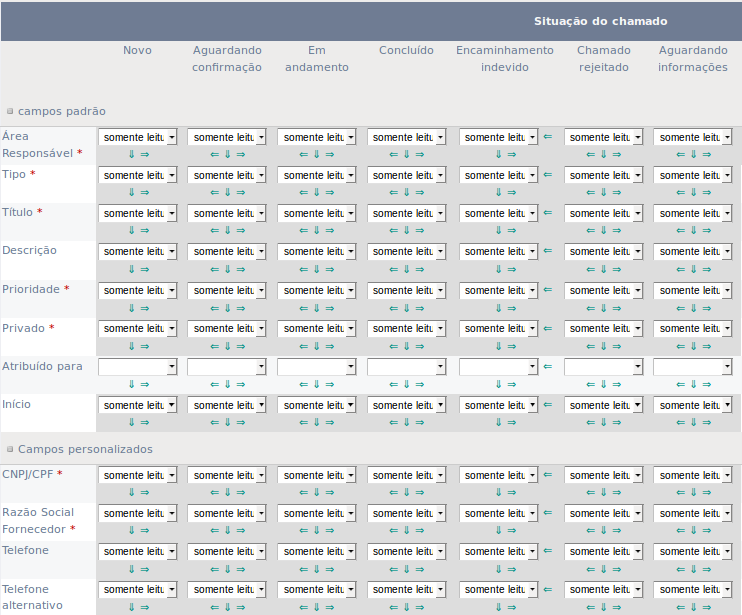
\includegraphics[width=1.0\textwidth]{imagens/workflow_fields.png}
  \caption{Tela de configuração de permissão de campos do fluxo de trabalho}
  \label{fig:redmine_campos}
\end{figure}

A transição de estados define para quais situações um chamado pode ser alterado de acordo com o estado atual, determinando para quais etapas de um processo um usuário consegue conduzir a tarefa. A Figura \ref{fig:redmine_transicoes} apresenta a tela de configuração das transições de estados no Redmine.

\begin{figure}[H]
  \centering
  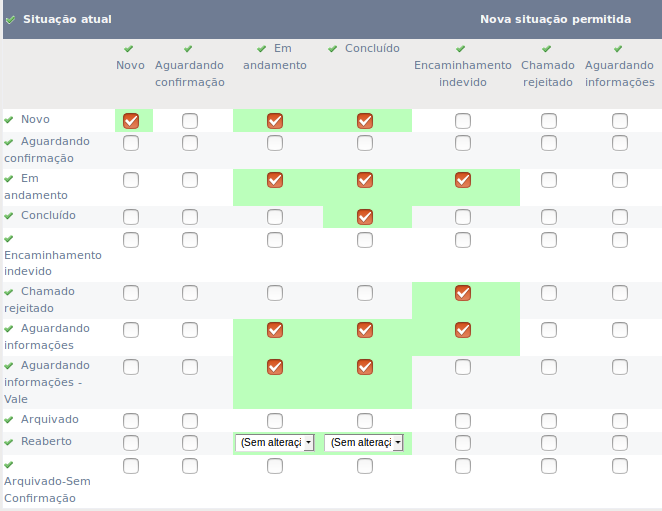
\includegraphics[width=1.0\textwidth]{imagens/workflow_status.png}
  \caption{Tela de configuração das transições de situação do fluxo de trabalho}
  \label{fig:redmine_transicoes}
\end{figure}

\subsection{Definição dos atores}\label{subsection:redmine-automatizar_processo-atores}

\subsubsection{Escolha dos atores}

Para definir que um \underline{usuário} poderá ser um ator de determinado processo, o mesmo deverá ser adicionado ao \underline{projeto} ao qual o \underline{tipo de tarefa} correspondente ao processo está relacionado. Esta operação exige que sejam também definidos os papéis que o usuário vai exercer nos processos deste projeto.

O papel que é dado ao usuário agrupa diferentes permissões. Dentre elas, é possível escolher se um usuário pode ter tarefas atribuídas a ele, quais tarefas ele consegue visualizar e quais ações ele é capaz de realizar sobre as tarefas, como ver, editar, criar, ou adicionar notas. As transições de estado de uma tarefa, bem como o controle de acesso aos campos das tarefas também estão incluídos neste conjunto de permissões, através do Fluxo de trabalho (\ref{subsection:redmine-fluxo_de_trabalho}), que é configurado dentro do papel.

\section{Precificação manual}\label{sec:redmine-impl-caso-uso}

Para implementar o caso de uso descrito na seção \ref{sec:introducao-caso_real} no Redmine, foi criado um \underline{tipo de tarefa} chamado Precificação manual. Também foram criadas as situações Novo, Solicitar troca de preço, Aguardando aprovação, Não aprovado, Trocar preço, Encerrado.

As situações acima representam cada etapa do processo. A transição de situação é feita pelo responsável pela tarefa naquele momento, que também altera para o novo responsável na próxima etapa, caso necessário. A etapa de troca de preço consiste da operação de um sistema externo, e assim que concluída, o responsável pela etapa atual, manualmente altera a situação da tarefa que representa o processo para "Encerrado", o que representa a conclusão da etapa de "Trocar Preço", e a conclusão do processo.

Esta implementação mostra como processos simples podem ser modelados no Redmine, se aproveitando de toda a sua estrutura de tarefas. Desta forma é possível que um usuário acompanhe processos, execute etapas manuais no processo, preenchendo formulários, e tomando decisões para as próximas etapas, como a etapa de aprovação.

A ferramenta escolhida se mostrou uma solução barata, de rápida implementação, e que permite que o próprio usuário administrador seja o responsável pela manutenção da mesma. 
Muitos cenários problemáticos como o de precificação manual, apresentado nesta seção, são simples e para que fluam melhor requerem uma padronização e automação mínima, que a utilização do Redmine pode oferecer.

\section{Cenário com aprovação paralela}\label{sec:cenario-complexo}

Apesar do grande potencial de configuração do Redmine que possibilita seu uso para automatização de processos simples, não é possível utilizá-lo em situações de maior complexidade. No exemplo utilizado, modelagem de processos é baseada em uma máquina de estados cujas transições são definidas apenas pelo estado atual do processo e do perfil de acesso dos usuários. Portanto, fluxos mais complexos que possuem, por exemplo, atividades executadas em paralelo ou regras de negócio dependentes de variáveis do contexto de cada execução de um processo não são possíveis de ser modelados apenas com as configurações padrão do Redmine.

Suponhamos que o processo descrito na Figura \ref{fig:exemplo_bpmn-problema} se tornasse um pouco mais complexo e a troca de preço precisasse ser aprovada por três gestores em paralelo, sendo que a reprovação de qualquer um deles reprovasse a precificação. Este caso já não é suportado pelo Redmine. No entanto, este sistema foi desenvolvido de forma a permitir a criação de funcionalidades complementares.

O Redmine foi projetado para ser extensível por meio de \textit{plugins}. Uma funcionalidade da ferramenta pode ser modificada, ou uma nova funcionalidade pode ser criada sem precisar alterar o código original do Redmine. Os \textit{plugins} são desenvolvidos em \textit{Rails}, o mesmo \textit{framework} de programação do Redmine. 

Para possibilitar extensões de funcionalidades que envolvem enxertar pedaços de código no meio de uma classe ou de uma tela, o Redmine disponibiliza \textit{hooks} em diversas partes da ferramenta. Hooks são \textit{tags} com um identificador da parte do código em que estão inseridas. Para utilizar um \textit{hook} basta incluir um \textit{hook} \textit{listener} num \textit{plugin}, e direcionar qual arquivo ou método um determinado \textit{hook} vai disparar.

Muitos plugins desenvolvidos pela comunidade estão disponíveis e podem ser usados para aumentar o poder de modelagem de processos, tornando o Redmine uma ferramenta ainda mais flexível. Esta facilidade nos permite estender o Redmine para possibilitar a implementação de processos mais complexos.

Existem plugins que permitem definir regras de aprovação, regras de mudança automática de etapas mediante eventos, e outros. No entanto, todos estes plugins são limitados, e consideram um contexto para o qual foram desenvolvidos. Para conduzir processos complexos contando apenas com o Redmine e diversos plugins, conforme a necessidade do processo, seria necessário um esforço muito grande para evoluir os plugins existentes, e criar alguns novos para demandas como disparar uma etapa automatizada que é realizada por outro sistema. 

O esforço de evoluir os plugins já existentes não é algo pequeno, pois são desenvolvidos por vários desenvolvedores da comunidade, e muitos daqueles não tem um código organizado ou legível, ou até mesmo não passam nos testes automatizados do Redmine.

A criação de novos plugins também é algo bastante custoso, não só pelo desenvolvimento do código em si, mas porque envolve garantir que cada novo plugin não quebre nenhum teste do Redmine, não gere nenhum problema para uma funcionalidade já existente, e também funcione perfeitamente bem em conjunto com os outros plugins.

O último ponto citado no parágrafo anterior nos leva ao principal obstáculo para que utilizemos apenas o Redmine com plugins para conduzir processos complexos: cada novo plugin adicionado ao conjunto de código original do Redmine adiciona um risco a mais para o funcionamento perfeito do sistema, podendo deixar a ferramenta cada vez mais instável. Portanto, não é indicado que uma mesma instância do Redmine rode em produção com uma quantidade muito grande de plugins, que é o que aconteceria se tivéssemos diversos plugins para atender a necessidade de processos complexos.

Pelas razões citadas acima, preferimos considerar sistemas consolidados que já foram desenvolvidos para gerenciamento de processos complexos, que além de atenderem as nossas necessidades, seriam bastante utilizados, e portanto bem testados. O capítulo \ref{chp:bpm} então introduzirá o conceito de BPM e os sistemas BPMS.